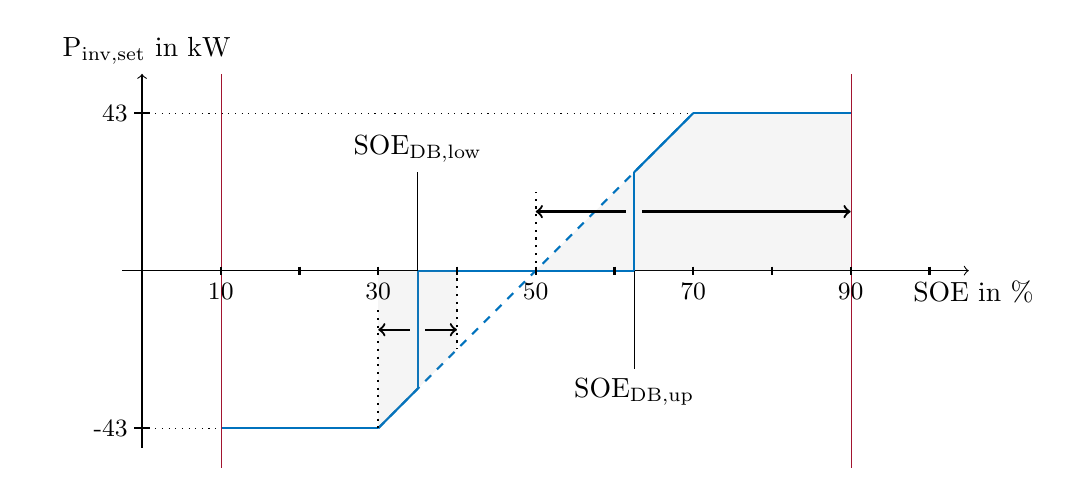
\begin{tikzpicture}

    %Define color for plot
    \definecolor{matlab_blue}{rgb}{0,0.4470,0.7410}
    \definecolor{matlab_darkred}{rgb}{0.6350,0.0780,0.1840}

    %Coordinates
    \coordinate (x30) at (3,2.5);
    \coordinate (x40) at (4,2.5);
    \coordinate (x50) at (5,2.5);
    \coordinate (x85) at (8.5,2.5);
    \coordinate (droop_x30) at (3,0.5);
    \coordinate (droop_x70) at (7,4.5);
    \coordinate (db_low) at (3.5,2.5);
    \coordinate (db_low_pow) at (3.5,1);
    \coordinate (db_high) at (6.25,2.5);
    \coordinate (db_high_pow) at (6.25,3.75);
    
    % Draw a grid
    %\draw[step=0.5cm,lightgray,ultra thin, opacity = 0.3] (-0.25,0.25) grid (9.25,5.25);
    
    % Draw a coordinate system
    \draw[thin,->] (-0.25,2.5) -- (10.5,2.5) node[rectangle,anchor=north] {
        \renewcommand{\arraystretch}{0.65}
        \begin{tabular}{c} 
            \normalsize SOE in \%
        \end{tabular}};
    
    \draw[thin,->] (0,0.25) -- (0,5) node[rectangle,anchor=south] {
        \renewcommand{\arraystretch}{0.65}
        \begin{tabular}{c} 
            \normalsize P\textsubscript{inv,set} in kW
        \end{tabular}};
    
    % Fill space below curve --> needed?
    \filldraw[draw=black, fill=gray!80,draw opacity=0,fill opacity=0.1] (5,2.5) -- (9,2.5) -- (9,4.5) -- (7,4.5) -- cycle;
    
    % Draw droop in blue dashed with solid endings
    \draw[thick,matlab_blue,dashed] (droop_x30) -- (droop_x70);
    \draw[thick,matlab_blue] (1,0.5) -- (droop_x30);
    \draw[thick,matlab_blue] (droop_x70) -- (9,4.5);
    
    % Draw adjusted droop including deadbands in solid
    \draw[thick,matlab_blue] (db_low) -- (db_high);
    \draw[thick,matlab_blue] (db_high) -- (db_high_pow);
    \draw[thick,matlab_blue] (db_high_pow) -- (droop_x70);
    
    \draw[thick,matlab_blue] (db_low) -- (db_low_pow);
    \draw[thick,matlab_blue] (db_low_pow) -- (droop_x30);
    
    % Draw range for adjusting upper deadband
    \draw[thick,dotted] (5,2.5) -- (5,3.5);
    \draw[thick,<-] (5,3.25) -- (6.15,3.25);
    \draw[thick,->] (6.35,3.25) -- (9,3.25);
    %\draw[very thin] (6.25,2.75) -- (6.5,2.75);
    \draw[very thin] (6.25,2.5) -- (6.25,1.25) node[rectangle,anchor=north] {\normalsize SOE\textsubscript{DB,up}};
    
    \filldraw[draw=black, fill=gray!80,draw opacity=0,fill opacity=0.1] (x30) -- (4,2.5) -- (4,1.5) -- (3,0.5) -- cycle;
    
    % Draw range for adjusting lower deadband
    \draw[thick,dotted] (3,2) -- (3,0.5);
    \draw[thick,dotted] (x40) -- (4,1.5);
    \draw[thick,<-] (3,1.75) -- (3.4,1.75);
    \draw[thick,->] (3.6,1.75) -- (4,1.75);
    %\draw[very thin] (3.5,2.25) -- (3.75,2.25);
    \draw[very thin] (3.5,2.5) -- (3.5,3.75) node[rectangle,anchor=south] {\normalsize SOE\textsubscript{DB,low}};
    
    % Draw physical limits of the battery
    \draw[ultra thin,matlab_darkred] (1,0) -- (1,5);
    \draw[ultra thin,matlab_darkred] (9,0) -- (9,5);
    \draw[thin,dotted] (0,4.5) -- (droop_x70);
    \draw[thin,dotted] (0,0.5) -- (1,0.5);
    
    % Draw ticks on the axes
    \draw[thick] (1,2.55) -- (1,2.45) node[pos=0.75, anchor=north] {\small 10};;
    \draw[thick] (2,2.55) -- (2,2.45);
    \draw[thick] (3,2.55) -- (3,2.45) node[pos=0.75, anchor=north] {\small 30};
    \draw[thick] (4,2.55) -- (4,2.45);
    \draw[thick] (5,2.55) -- (5,2.45) node[pos=0.75, anchor=north] {\small 50};
    \draw[thick] (6,2.55) -- (6,2.45);
    \draw[thick] (7,2.55) -- (7,2.45) node[pos=0.75, anchor=north] {\small 70};
    \draw[thick] (8,2.55) -- (8,2.45);
    \draw[thick] (9,2.55) -- (9,2.45) node[pos=0.75, anchor=north] {\small 90};
    \draw[thick] (10,2.55) -- (10,2.45);
    
    \draw[thick] (-0.1,4.5) -- (0.1,4.5) node[pos=0.25, anchor=east] {\small 43};
    \draw[thick] (-0.1,0.5) -- (0.1,0.5) node[pos=0.25, anchor=east] { \small -43};
    
\end{tikzpicture}